\documentclass[a4paper,titlepage]{article}
\usepackage{ascmac}
\usepackage{amsmath,amssymb}
\usepackage{siunitx}
\sisetup{group-separator = {,}}
\usepackage[dvipdfmx]{graphicx}

\usepackage{listings}
\usepackage{color}

\lstset{
language={Ruby},
basicstyle={\small\ttfamily},
identifierstyle={\small},
commentstyle={\small\ttfamily \color[rgb]{0,0.5,0}},
keywordstyle={\small\ttfamily\bfseries \color[rgb]{1,0,0}},
ndkeywordstyle={\small},
stringstyle={\small\ttfamily \color[rgb]{0,0,1}},
frame={tb},
breaklines=true,
columns=[l]{fullflexible},
numbers=left,
xrightmargin=0zw,
xleftmargin=3zw,
numberstyle={\scriptsize},
stepnumber=1,
numbersep=1zw,
morecomment=[l]{//}
}

\newcommand{\Cost}{\mathrm{Cost}}
\newcommand{\Price}{\mathrm{Price}}
\newcommand{\Power}{\mathrm{Power}}
\newcommand{\toluene}{\mathrm{toluene}}
\newcommand{\coolant}{\mathrm{coolant}}
\newcommand{\steam}{\mathrm{steam}}
\newcommand{\reactor}{\mathrm{reactor}}

\begin{document}
  \title{Process System Engineering \#6}
  \author{\#03150796 Amane Suzuki}
  \date{November 10, 2015}
  \maketitle

  \section{Abstract}
  I use the Simplex Method to find the best conditions of this plant.
  Simplex Method has enough performance and it can calculate the best conditions.

  \section{Algorithm}
  Figure \ref{fig:simplex} shows a flow of Simplex Method.

  \begin{figure}[htbp]
    \centering
    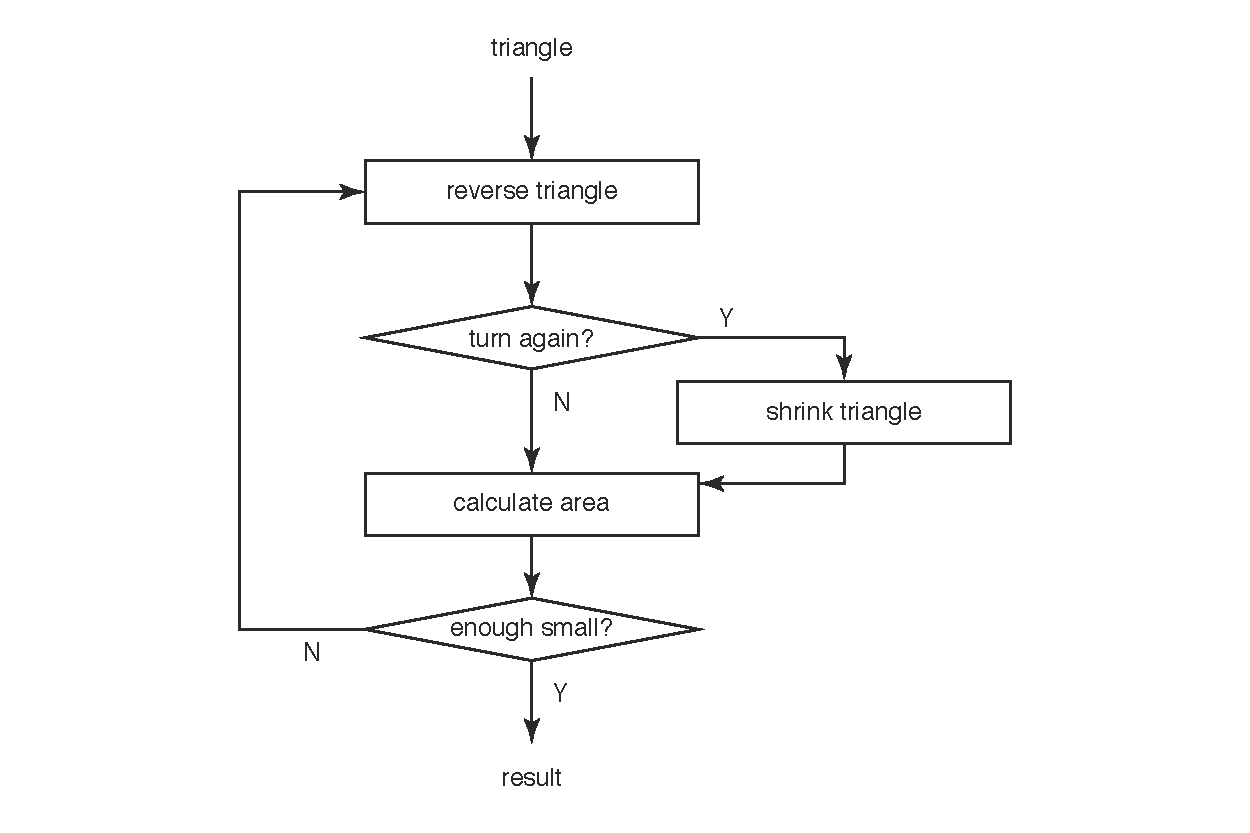
\includegraphics[width=12cm]{images/simplex.pdf}
    \caption{The flow chart of Simplex Method.}
    \label{fig:simplex}
  \end{figure}

  Simplex Method is faster than Steppest Decent Method (I used last week).
  Processing time is about $0.5 \si{\second}$.

  \section{Result and Discussion}
  Table \ref{tb:result} shows the best conditions in $N=1, 2, 3, 4, 5$.
  \begin{table}[htbp]
    \centering
    \begin{tabular}{llllll}\\\hline
      & $N=1$ & $N=2$ & $N=3$ & $N=4$ & $N=5$ \\\hline
      $\gamma_0$ [wt\%] & 0.0727 & 0.0969 & 0.1 & 0.1 & 0.1 \\\hline
      Coolant Temperature [\si{\kelvin}]& 253.0 & 253.0 & 261.0 & 266.5 & 271.1 \\\hline
      Total Cost [\si{\yen\per\second}] & 42.89 & 30.45 & 28.05 & 27.45 & 27.27\\\hline
%      Processing Time [\si{\second}] & 0.47 & 0.73 & 0.23 & 0.40 & 0.59 \\\hline
    \end{tabular}
    \caption {The best conditions from N=1 to N=5}
    \label{tb:result}
  \end{table}

  Except $N=1, 2$, the best $\gamma_0$ is $0.1$. It is because steam cost is dominant in total cost.
  In $N=1, 2$, however, too large $\gamma_0$ makes power consumption infinite. So best $\gamma_0$ are $0.0727$
  and $0.0969$.

  The result suggest us to make plant in $N=5, \gamma_0=0.1, T_2 = 271.1$.
  Thinking realistically, however, we should consider the area of land, plant stability, and ease of control.


  \newpage
  \section{Source Program}
  \lstinputlisting[caption=main.rb, label=code:main]{code/main.rb}
  \newpage
  \lstinputlisting[caption=plant.rb, label=code:plant]{code/plant.rb}
  \newpage
  \lstinputlisting[caption=reactor.rb, label=code:reactor]{code/reactor.rb}
  \newpage
  \lstinputlisting[caption=optimize.rb, label=code:optimize]{code/optimize.rb}
\end{document}
